	\chapter*{Resultados}
\addcontentsline{toc}{chapter}{Resultados}

Através da função de construção de gráficos mencionado anteriormente, foi possível construir diversos gráficos para a comparação de métodos, funções de correlação e os resultados entre as bibliotecas usando o traçador \textit{NumberCountTracer}. 

\subsection*{Comparação dos cálculos do CCL usando os dados do caso de histograma}

Ao comparar os cálculos realizados com mesma função de correlação usando os métodos \textit{fftlog} e \textit{bessel}, os dados do caso de histograma obtemos os seguintes gráficos.

\begin{figure}[h!]
	\centering
	\caption{Comparação entre os métodos \textit{fftlog} e o \textit{bessel} para a mesma função de correlação no caso de histograma.}
	\label{fig:fig1}
	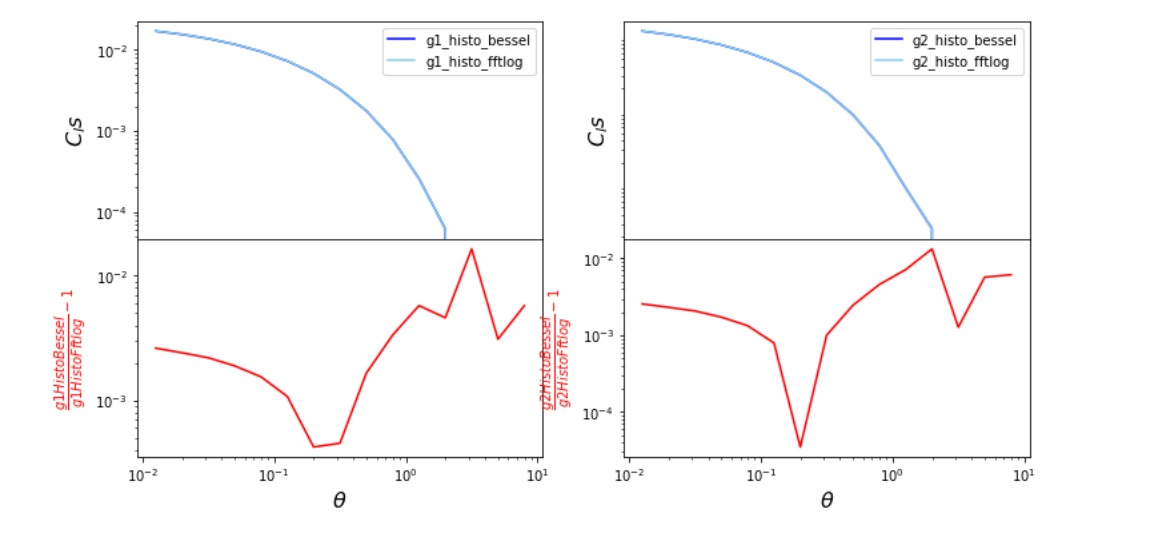
\includegraphics[width=0.7\linewidth]{figuras/fig1}
	
	Fonte: O jupyter notebook \textit{NumCosmoCCLTest\_Cross-Correlation.ipynb}.
\end{figure}

As curvas plotadas nos primeiros gráficos mostram que os cálculos convergem e a distância relativa entre os valores calculados utilizando métodos diferentes concordam entre si com uma precisão média de $ 10^{-3} $ entre os valores calculados. 

\newpage
Em seguida, ao comparar as curvas dos cálculos com funções de correlação diferentes com o mesmo método e os dados de histograma obtemos o seguinte gráfico:

\begin{figure}[H]
	\centering
	\caption{Comparação os mesmos métodos e diferentes funções de correlação no caso de histograma.}
	\label{fig:fig2}
	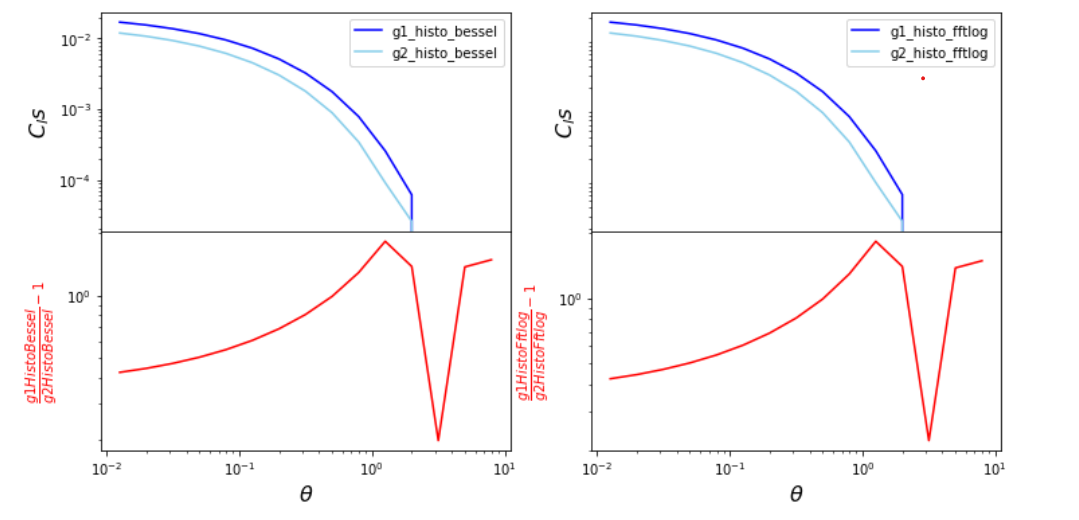
\includegraphics[width=0.7\linewidth]{figuras/fig2}
	
	Fonte: O jupyter notebook \textit{NumCosmoCCLTest\_Cross-Correlation.ipynb}.
\end{figure}

As curvas dos cálculos plotados nos primeiros gráficos não convergem para os mesmos pontos, porém possuem o mesmo comportamento. A distância relativa entre os valores calculados utilizando os mesmos métodos em diferentes funções de correlação possuem pouca concordância entre si com uma precisão média de $ 10^0 $.

\subsection*{Comparação dos cálculos do CCL usando os dados do caso analítico}

Ao comparar os cálculos realizados com mesma função de correlação usando os métodos \textit{fftlog} e \textit{bessel}, os dados do caso analítico, obtemos os seguintes gráficos. 

\begin{figure}[H]
	\centering
	\caption{Comparação entre os métodos \textit{fftlog} e o \textit{bessel} utilizando os dados do caso analíticos.}
	\label{fig:fig3}
	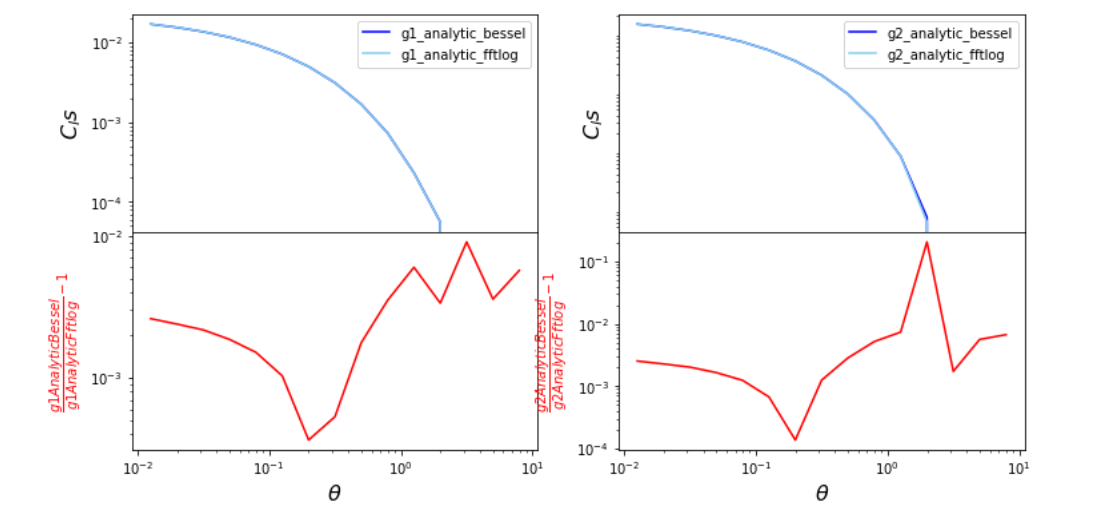
\includegraphics[width=0.7\linewidth]{figuras/fig3}
	
	Fonte: O jupyter notebook \textit{NumCosmoCCLTest\_Cross-Correlation.ipynb}.
\end{figure}

As curvas plotadas nos primeiros gráficos mostram que os cálculos convergem e a distância relativa entre os valores calculados utilizando métodos diferentes concordam entre si com uma precisão média de $ 10^{-3} $ entre os valores calculados. Por fim, comparamos os mesmos métodos para diferentes funções de correlação e obtemos os seguintes gráficos:

\begin{figure}[H]
	\centering
	\caption{Comparação dos mesmos métodos para calcular funções de correlação diferentes utilizando os dados do caso analítico.}
	\includegraphics[width=0.7\linewidth]{"figuras/fig4"}
	
	\label{fig:fig4}
	
	Fonte: O jupyter notebook \textit{NumCosmoCCLTest\_Cross-Correlation.ipynb}.
\end{figure}

A distância relativa na quarta análise demostra que os resultados apresentam pouca precisão e pouca concordância entre si, mas segue um comportamento semelhante.

\subsection*{Comparação entre os resultados do CCL e da NumCosmo}

Para a comparação entre os cálculos da NumCosmo e do CCL, usamos os resultados calculados pela NumCosmo com o método \textit{CVODE} e o conjunto de dados do caso de histograma, comparando uma função de correlação por vez, usando o mesmo método e função de correlação por ambas as bibliotecas e assim obtemos os seguintes gráficos: 

\begin{figure}[H]
	\centering
	\caption{Comparação dos cálculos usando o método \textit{bessel} e a função de correlação g1 por ambas as bibliotecas.}
	\includegraphics[width=0.7\linewidth]{"figuras/fig5"}	
	\label{fig:fig5}
	
	Fonte: O jupyter notebook \textit{NumCosmoCCLTest\_Cross-Correlation.ipynb}.
\end{figure}

\begin{figure}[H]
	\centering
	\caption{Comparação dos cálculos usando o método \textit{fftlog} e a função de correlação g1 por ambas as bibliotecas.}
	\includegraphics[width=0.7\linewidth]{"figuras/fig6"}	
	\label{fig:fig6}
	
	Fonte: O jupyter notebook \textit{NumCosmoCCLTest\_Cross-Correlation.ipynb}.
\end{figure}

\begin{figure}[H]
	\centering
	\caption{Comparação dos cálculos usando o método \textit{bessel} e a função de correlação g2 por ambas as bibliotecas.}
	\includegraphics[width=0.7\linewidth]{"figuras/fig7"}	
	\label{fig:fig7}
	
	Fonte: O jupyter notebook \textit{NumCosmoCCLTest\_Cross-Correlation.ipynb}.
\end{figure}

\begin{figure}[H]
	\centering
	\caption{Comparação dos cálculos usando o método \textit{fftlog} e a função de correlação g2 por ambas as bibliotecas.}
	\includegraphics[width=0.7\linewidth]{"figuras/fig8"}	
	\label{fig:fig8}
	
	Fonte: O jupyter notebook \textit{NumCosmoCCLTest\_Cross-Correlation.ipynb}.
\end{figure}

Os primeiros gráficos apresentados por ambas as figuras mostram que os resultados obtidos pelas bibliotecas convergem, isto é, foi possível mostrar a concordância entre os resultados das duas bibliotecas através dos gráficos de distância relativa que os resultados se aproximam com uma precisão da ordem de $ 10^{-4} $. 